\section{Particle-Hole Response and Polarization Propagator}
%\markright{Particle-Hole Response \ldots}
\subsection{Bethe-Salpeter Equation for the Polarization Propagator}
%
To investigate the dynamic properties of many-body systems, these systems
may be exposed to an external probe,
usually a one-body operator in second quantized form (see (\ref{eq:H1}))
%
	\begin{equation}
		\opO
	=
		\sum_{\alpha\beta}
		\ME<\alpha|\opOhatless|\beta> \Oc{\alpha} \Oa{\beta}
	\;.
	\label{eq:opO}
	\end{equation}
%
Examples of such operators are the electric and magnetic multipole operators
or the Gamow-Teller charge-exchange operator.
In the case of charge-exchange $\Oa{\beta}$ should annihilate a proton while
$\Oc{\alpha}$ creates a neutron (or the isospin should be included in the 
quantum numbers $\alpha$ and $\beta$).
The response to an operator of the form (\ref{eq:opO}) is expressed in the 
form of the excitation strength distribution
%
	\begin{equation}
		S_\opO(\omega)
	=
		\sum_n
		\left|
			\ME<\Psi_n|\opO|\Psi_0>
		\right|^2
		\delta(\omega-(E^n-E^0)) 
	\label{eq:SopO}
	\;,
	\nonumber \\
	\end{equation}
%
where the index $n$ labels the excited states including the continuum and 
$|\Psi_0\rangle$ is the ground state of the many-body system, \ie\ the exact
ground state of the full Hamiltonian $\hat{H}$ (\ref{eq:Hamiltonian}). 
The response function may be re-expressed as
%
\begin{equation}
		S_\opO(\omega)
	=
		-\frac{1}{\pi}
		\;
		{\rm Im}
		\;
		\sum_{\alpha\beta\gamma\delta}
		\ME<\alpha|\opOhatless|\beta>^*
		L_{\alpha\beta;\gamma\delta}(\omega)
		\ME<\gamma|\opOhatless|\delta>
	\;.
	\label{eq:defS}
	\end{equation}
%
Here the polarization propagator $L$ defined as
%
	\begin{eqnarray}
		L_{\alpha\beta;\gamma\delta}(\omega)
	&=&
		\sum_{n\not=0}
		\left[
			\frac{\ME<\Psi_0|\Oc{\beta}  \Oa{\alpha}|\Psi_n>
			      \ME<\Psi_n|\Oc{\gamma} \Oa{\delta}|\Psi_0>
			}
			{\omega-(E^n-E^0)+i\eta}
		\right] 
	\nonumber \\
	&-&
		\sum_{m\not=0}
		\left[
			\frac{\ME<\Psi_0|\Oc{\gamma} \Oa{\delta}|\Psi_m>
			      \ME<\Psi_m|\Oc{\beta}  \Oa{\alpha}|\Psi_0>
			}
			{\omega-(E^0-E^m)-i\eta}
		\right]
	\label{eq:DefLLeh}
	\end{eqnarray}
%
is introduced. The polarization propagator contains information on
excitations due to the action of $\opO$ and de-excitation due to 
$\opO^\dagger$. In the case of a charge-exchange operator 
the  initial and the final nucleus are not the same.
Information
about $(p,n)$ as well as $(n,p)$ reactions is contained in $L$.
The calculation of the response function for the charge-exchange 
is treated in chapter~\ref{chap:DERPA}. 

The second line of (\ref{eq:DefLLeh}) does not contribute to the strength 
distribution
(\ref{eq:defS}), but it contains information according to response to the
conjugate operator $\opO^\dagger$, and is 
added, because now $L(\omega)$ (\ref{eq:DefLLeh}) can be identified as the 
Fourier transform
of the polarization propagator
%
	\begin{eqnarray}
		iL_{\alpha\beta;\gamma\delta}(t-t')
	&=&
		\ME<\Psi_0|
		T\left[
			\Oc{\beta}(t)\Oa{\alpha}(t)
			\Oc{\gamma}(t')\Oa{\delta}(t')
		\right]
		|\Psi_0>
	\nonumber \\
	&-&
		\ME<\Psi_0|\Oa{\alpha}(t)\Oc{\beta}(t)|\Psi_0>
		\ME<\Psi_0|\Oa{\delta}(t')\Oc{\gamma}(t')|\Psi_0>
	\label{eq:DefL}
	\;,
	\end{eqnarray}
%
in which $T$ is (again) the time-ordering operator (\cf\ (\ref{eq:g1t})). 

As will be shown in appendix~\ref{app:detail}, the quantity 
$\ME<\alpha|\opOhatless|\beta>$ can be calculated if the basis is chosen, so
the polarization propagator contains all essential
information about one-body excitations of the system to linear approximation
in the probing field. 
The polarization propagator
$L$ is a special case of the three-times response propagator\cite{BAD90}
%
	\begin{eqnarray}
		i\tilde{L}_{\alpha\beta;\gamma\delta}(t_1-t',t_2-t')
	&=&
		\ME<\Psi_0|
		T\left[
		\Oc{\beta}(t_2)\Oa{\alpha}(t_1)
		\Oc{\gamma}(t')\Oa{\delta}(t')
		\right]
		|\Psi_0>
	\label{eq:DefLt} \\
	&-&
		\ME<\Psi_0|\Oa{\alpha}(t_1)\Oc{\beta}(t_2)|\Psi_0>
		\ME<\Psi_0|\Oa{\delta}(t')\Oc{\gamma}(t')|\Psi_0>
	\nonumber
	\end{eqnarray}
%
Analogous to the derivation of the Dyson equation (\ref{eq:Dyson}),
the equation of motion for the three-times propagator (\ref{eq:DefLt}) leads
to  the following Bethe-Salpeter 
equation\cite{BK61} (BSE). 
%
%
	\begin{eqnarray}
		\lefteqn{\tilde{L}_{\alpha\beta;\gamma\delta}(t_1-t_2,t'_1-t_2)
	=
		-ig_{\alpha\gamma}(t_1-t_2)g_{\delta\beta}(t_2-t'_1)
	}
	\label{eq:BS} \\
	&+&
		\sum_{\mu\nu\kappa\lambda}
		%\int\!\!\!\!\int\!\!\!\!\int\!\!\!\!
		\int {\rm d}t_3 {\rm d}t_4 {\rm d}t_5 {\rm d}t_6
		\Bigl[
			-i\;g_{\alpha\mu}(t_1-t_3)g_{\nu\beta}(t_4-t'_1)
	\nonumber\\
	&\times&
		i\Gamma_{\mu\nu;\kappa\lambda}^{ph}(t_3,t_4;t_5,t_6)
		\;\tilde{L}_{\kappa\lambda;\gamma\delta}(t_5-t_2,t_6-t_2)
		\Bigr] \;,
	\nonumber
	\end{eqnarray}
%
in which $g$ is the one-body propagator defined in eq.~(\ref{eq:g1t})
which solves the Dyson equation (\ref{eq:Dyson}) (fig.~\ref{fig:Dyson}).
Eq.~(\ref{eq:BS}) is graphically displayed in fig.~\ref{fig:BSE}.
%%%%%%%%%%%%%%%%%
\begin{figure}
\centerline{
\epsfig{file=figures/BSEph.eps,height=4cm}
}
\caption[]{
Graphical representation of the Bethe-Salpeter equation (\ref{eq:BS}).
\label{fig:BSE}}
\end{figure}
%%%%%%%%%%%%%%%%%

%
In (\ref{eq:BS}) $\Gamma^{ph}_{\mu\nu;\kappa\lambda}(t_3,t_4;t_5,t_6)$
plays the role of an effective particle-hole interaction in analogy with 
the quantity $\Sigma_{\gamma\delta}^\ast$ in the Dyson equation, 
which acts as an effective
potential, non-local in space and time, in which the particles propagate.
In the framework of the theory of linear response it has been shown 
that, in order to 
satisfy conservation laws (gauge invariance, sum rules), 
a relation should be maintained between 
the effective potential $\Sigma^\ast$ and the effective interaction $\Gamma$;
this Baym-Kadanoff condition\cite{BK61,Ba62} is formally expressed by the 
functional derivative
%
	\begin{equation}
		\Gamma_{\alpha\beta;\gamma\delta}
	=
		\frac{
			\delta \Sigma_{\alpha\beta}^\ast
		}{
			\delta g_{\gamma\delta}
		}
	\;.
	\label{eq:BK}
	\end{equation}
%
The implications that of the BK-condition (\ref{eq:BK}) for the HF and the
second-order self-energy are  displayed in figs.~\ref{fig:SGHF} 
and~\ref{fig:SG2nd}.
%%%%%%%%%%%%%%
\begin{figure}
\centerline{
\hbox to 8cm{
\cntrbox{2cm}{1cm}{\epsfig{ file=figures/selfenergy/sig_HF.ps, width=2cm}}
\hfill
\cntrbox{2cm}{1cm}{\epsfig{ file=figures/gamma/gam_HF.ps, width=2cm}}
}}
\caption[]{Diagram of the HF self-energy $\Sigma^\ast$ (left). 
The thick line represent a dressed propagator, \ie\ solutions of 
(\ref{eq:Dyson}). The figure on the right is the contribution
to $\Gamma^{ph}$ as constructed with the Baym-Kadanoff condition (\ref{eq:BK}).
\label{fig:SGHF}}
\end{figure}
%%%%%%%%%%%%%%
%%%%%%%%%%%%%%
\begin{figure}
%
% gamma sigma figure 2nd
%
\setbox1=\vbox{
\hbox{\epsfig{ file=figures/gamma/gam_2ndorder_pp.ps, width=2cm}}
\hbox{\epsfig{ file=figures/gamma/gam_2ndorder_ph.ps, width=2cm}}
}
\dimen1=\ht1
\centerline{
\hbox to 8cm{
\vbox to \ht1{
     \vfill
     \hbox{\epsfig{ file=figures/selfenergy/sig_2nd.ps, width=2cm}}
     \vfill}
\hfill
\hbox{\box1}
}}
\caption[]{Same figure as fig.~\ref{fig:SGHF}, but for the second-order 
self-energy.
\label{fig:SG2nd}}
\end{figure}
%%%%%%%%%%%
Eq.~(\ref{eq:BS}) describes the summation of all possible diagrams. A 
brute force numerical treatment based upon approximations for the self-energy
resulting in approximations for the particle-hole vertex through the 
condition (\ref{eq:BK})
is out of reach for the present computers. Therefore approximations have been 
proposed, inspired by the physical processes described by the diagrams.  In
this line of research dominant processes can be identified.

The BSE (\ref{eq:BS}) reduces to an equation for $L$ if $\Gamma$ contains a 
factor
$\delta(t_5-t_6)$. If this is not the case, the full $\tilde{L}$ has to be
calculated and in the end the limit $t_1 \rightarrow t_2$ should be taken.
In practical situations\cite{BAD90} (\ref{eq:Dyson}) is solved
in some approximation for $\tilde{\Gamma}$, that the equation 
under consideration directly yields $L$
%
	\begin{eqnarray}
	\lefteqn{
		L_{\alpha\beta;\gamma\delta}(t_1-t_2)
	=
		-ig_{\alpha\gamma}(t_1-t_2)g_{\delta\beta}(t_2-t_1) 
	+
	\mbox{ }
	}
	\label{eq:BSap} \\
	&&
	\hspace{-0.5cm}
		\sum_{\mu\nu\kappa\lambda}
		%\int\!\!\!\!\int\!\!\!\!\int\!\!\!\!
		\int dt_3dt_4%dt_5dt_6
		\Bigl[
		-i\;g_{\alpha\mu}(t_1-t_3)g_{\nu\beta}(t_3-t_1)
	%
		i\tilde{\Gamma}_{\mu\nu;\kappa\lambda}(t_3,t_4)
		\;L_{\kappa\lambda;\gamma\delta}(t_4-t_2)
		\Bigr] 
	\nonumber
	\;.
	\end{eqnarray}
%
%%%%%%%%%%
%
\subsection{Random Phase and Various Other Approximations}
The starting point for an approximate description of response based on the 
BSE (\ref{eq:BS}) is
some mean-field approximation for the effective single-particle potential
$\Sigma^\ast$ that yields bound state solutions. A well-known way to produce 
such a potential is the Hartree-Fock (HF) approximation\cite{RS80}. This 
corresponds
to solving the Dyson equation (\ref{eq:DysonE}) with a $\Sigma^\ast$ that is 
of the form fig.~\ref{fig:SGHF}. The single-particle propagator is then given 
by the expression (\cf\ (\ref{eq:g10}))
%
	\begin{equation}
		g^{HF}_{\alpha\beta}(\omega) 
	=
		\delta_{\alpha\beta}
		\left[
			\frac{\theta(\alpha-F)}
			{\omega - \varepsilon^{HF}_\alpha + i \eta}
	+
			\frac{\theta(F-\alpha)}
			{\omega - \varepsilon^{HF}_\alpha - i \eta}
		\right]
	\label{eq:gHF}
	\end{equation}
%
where $\varepsilon^{HF}_\alpha$ are the Hartree-Fock single-particle 
energies (\ref{eq:SPE}).

\subsubsection{RPA}
With the HF approximation for the self-energy $\Sigma^\ast$, 
according to the Baym-Kadanoff condition (\ref{eq:BK}), the effective 
particle-hole interaction should be taken to be
$\Gamma_{\alpha\beta\gamma\delta} = V_{\alpha\beta\gamma\delta}$.
Due to their static, \ie\ energy-independent nature of both
$\Sigma^\ast$ and $\Gamma$, the Bethe-Salpeter equation (\ref{eq:BS}) is now 
drastically simplified to the Random Phase Approximation (RPA) equation
(with omission of the summation sign, using Einsteins summation convention 
that repeated indices should be summed over)
%
	\begin{equation}
		L^{\mbox{\tiny RPA}}_{\alpha\beta;\gamma\delta}(\omega)
	=
		L^0_{\alpha\beta;\gamma\delta}(\omega)
	+
		\sum_{\kappa\lambda\mu\nu}
		L^0_{\alpha\beta;\kappa\lambda}(\omega)
		V_{\kappa\lambda;\mu\nu}
		L^{\mbox{\tiny RPA}}_{\mu\nu;\gamma\delta}(\omega)
	\label{eq:RPA}
	\end{equation}
%
with
%
	\begin{eqnarray}
	\lefteqn{
		L^0_{\alpha\beta;\gamma\delta}(\omega)
	=
		\int\frac{d\omega'}{2\pi i}
		g^{HF}_{\alpha\gamma}(\omega+\omega')
		g^{HF}_{\delta\beta}(\omega')
	}&&\\
	&=&
		\delta_{\alpha\gamma}
		\delta_{\beta\delta}
		\left[
			\frac{\theta(\alpha-F)\theta(F-\beta)}
			{\omega - 
			(\varepsilon^{HF}_\alpha - \varepsilon^{HF}_\beta)
                        + i \eta}
	-
			\frac{\theta(F-\alpha)\theta(\beta-F)}
			{\omega - 
			(\varepsilon^{HF}_\alpha - \varepsilon^{HF}_\beta)
                        - i \eta}
		\right]
	\nonumber
	\;.
	\end{eqnarray}
%
The energies $\varepsilon^{HF}_\alpha$ that appear in the HF 
propagator (\ref{eq:gHF}) can be replaced by empirical ones, when 
those from a HF calculation are unsatisfactory.

In a discrete basis the RPA equation for the propagator $L$ leads to a 
homogeneous set of equations for the amplitudes
%
	\begin{subeqnarray}
		X^n_{\alpha\beta} 
	&=&
		\ME<\Psi_0|\Oc{\beta}  \Oa{\alpha}|\Psi_n>
	\\
		Y^m_{\alpha\beta} 
	&=&
		\ME<\Psi_0|\Oc{\alpha} \Oa{\beta}|\Psi_m>
	\end{subeqnarray}
%
which can be solved by standard matrix manipulations. 
The well-known symmetry ($\omega\rightarrow-\omega$; $X\leftrightarrow Y$) for 
the RPA solutions no longer exists for charge-exchange excitations. In the 
latter case the forward and backward going amplitudes correspond to 
($p$,$n$) and ($n$,$p$) amplitudes, respectively. 
This case will be treated in chapter~\ref{chap:DERPA}.

For the case of an energy continuum of excited states it is more appropriate 
to write (\ref{eq:RPA}) in the form
%
	\begin{equation}
		\left( 
		L^{\mbox{\tiny RPA}\phantom{0}}(\omega)
		\right)^{-1}_{\alpha\beta\gamma\delta}
	=
		\left( 
		L^{0}(\omega)
		\right)^{-1}_{\alpha\beta\gamma\delta}
	-
		V_{\alpha\beta\gamma\delta}
	\label{eq:RPAinv}
	\;,
	\end{equation}
%
in which the singular behavior of the propagators $L$ may be removed by 
giving the infinitesimal $\eta$ in (\ref{eq:DefLLeh}) and (\ref{eq:gHF})
a finite value. Thereby the strength distribution (\ref{eq:defS}) becomes a sum
of Lorentzians, rather than delta-functions, which is more convenient for
plotting purposes, and more in line with finite experimental energy resolution.
The methods of solving RPA-like equations are given in section~\ref{sec:RPAsol}.

Physically the RPA corresponds to a small-amplitude (harmonic) approximation 
of oscillations around a mean-field configuration. If the energy of the 
collective oscillation becomes small or imaginary, one should expect 
a transition to a phase distinct from that of the adopted mean field. 
In that case one must resort to higher-order terms for the polarization 
propagator, 
\eg\ the Extended RPA of ref.~\cite{BAD90}.

\subsubsection{ERPA}
The clear evidence of the fragmentation of one-hole strength requires a 
description of the single-particle propagator with at least a second-order 
self-energy (see fig.~\ref{fig:SG2nd}). The Baym-Kadanoff condition then 
dictates a particle-hole vertex $\Gamma^{ph}$ of the form given on the right
hand side of fig.~\ref{fig:SG2nd}. This form of $\Gamma^{ph}$ is approximately
introduced in the so-called Extended RPA (ERPA) approach\cite{BAD90}. 

This extension had been found to be essential for low-energy isoscalar 
excitations. 
The G-matrix interaction had turned out to be so strong that in large model 
spaces 
the most collective excitations had got imaginary eigenvalues. A counteracting 
effect is the weakening of the effective force by `screening', \ie\ interaction
via virtual excitations of the medium (fourth diagram in 
fig.~\ref{fig:ERPAdiagrams}). For isovector excitations this `screening' 
diagram had made the repulsive interaction even somewhat stronger rather than 
weaker as the word suggests\cite{BAD90}. In order to obey the Baym-Kadanoff 
condition (\ref{eq:BK}), and thereby conservations laws, also the other 
second-order diagrams of fig.~\ref{fig:ERPAdiagrams} must be included.
The second and third, called `self-screening', diagrams account to some extent 
for the fragmentation of the single-particle strength by the dressing of the 
propagator. A method which emphasizes this aspect is discussed in the next 
section.

The ERPA equation is similar to the RPA equation (\ref{eq:RPA}), 
with the difference that
an effective energy-dependent interaction is introduced
(using Einsteins convention again):
%
	\begin{equation}
		L^{\mbox{\tiny ERPA}}_{\alpha\beta;\gamma\delta}(\omega)
	=
		L^0_{\alpha\beta;\gamma\delta}(\omega)
		+%\sum_{\kappa\lambda\mu\nu}
		L^0_{\alpha\beta;\kappa\lambda}(\omega)
		\Gamma^{\mbox{\tiny ERPA}}_{\kappa\lambda;\mu\nu}(\omega)
		L^{\mbox{\tiny ERPA}}_{\mu\nu;\gamma\delta}(\omega)
	\label{eq:ERPA}
	\;.
	\end{equation}
%
This ERPA equation can be derived from the general form (\ref{eq:BS}) of the BS
equation with some simplifying assumptions \cite{BAD90}. 
Firstly, it is assumed, 
that the one-particle propagators $g$ have the single-pole structure 
(\ref{eq:gHF}) and the index pairs $\alpha\beta$ and $\gamma\delta$ refer 
only to particle-hole or hole-particle pairs. 
Secondly, the interaction $\Gamma$ is only expanded to second order in $V$, 
while also terms of $\Sigma^\ast$ to second order in $V$ are included in 
$\Gamma$, which consequently depends on just one energy variable. 
This method implies that the diagrams in fig.~\ref{fig:ERPAdiagrams}
are present in the summation.
%
% figuur
%
\begin{figure}
\centerline{
\epsfig{figure=figures/erpa/RPA2ndorder.ps, height=.65in}\hspace{25pt}
\epsfig{figure=figures/erpa/selfscr1.ps,    height=.65in}\hspace{25pt}
\epsfig{figure=figures/erpa/selfscr2.ps,    height=.65in}\hspace{25pt}
\epsfig{figure=figures/erpa/screening.ps,   height=.65in}\hspace{25pt}
\epsfig{figure=figures/erpa/ladder.ps,      height=.65in}
}
\caption[]{All diagrams of second order in $V$ (wiggly line) that start
with a particle-hole state and end with a particle-hole state. The arrows
denote single-pole propagators ($g^{HF}$). The first diagram is already
taken into account in the RPA equation. The second and third diagrams
are called%
\cite{BAD90} self-screening. The fourth is the screening diagram. Number
five is the ladder diagram.
\label{fig:ERPAdiagrams}}
\end{figure}
%%%%%%%%%%%%%
The fact that these diagrams
can be included via an equation like (\ref{eq:ERPA}) is not trivial. 
It can only be seen by writing out the expressions in detail.

%\typeout{checkitout}
%If the calculation is carried out straightforwardly a term $A L^0$ is
%accompanying $L^0\tilde{V}L^0$, with $A$ a diagonal matrix. But $A$ is small, 
%in the order of $1\%$, and therefore this term was neglected.

Due to the energy-dependence of $\Gamma$ normalization of the amplitudes
$X$ and $Y$ is not the same as in RPA. A treatment of the normalization 
condition is given in refs.~\cite{HDA86,AEG93}.

\subsubsection{DRPA}
An unsatisfactory feature of the ERPA is that no amplitudes $X_{\alpha\beta}$
and $Y_{\alpha\beta}$ are included for index pairs $\alpha\beta$  or 
$\gamma\delta$ which are of particle-particle or hole-hole nature, \ie\
of both orbits above or both below the Fermi level. That such contributions 
to the nuclear response may be most relevant has been demonstrated with the 
strength distribution for charge-exchange ($n,p$) reactions on magic nuclei 
with neutron excess.
To describe such phenomena the so-called Dressed RPA (DRPA) was 
introduced\cite{RGBA93} with the equation
%
	\begin{equation}
		L^{\mbox{\tiny DRPA}}_{\alpha\beta;\gamma\delta}(\omega)
	=
		L^f_{\alpha\beta;\gamma\delta}(\omega)
	+
		%\sum_{\kappa\lambda\mu\nu}
		L^f_{\alpha\beta;\kappa\lambda}(\omega)
		\Gamma^{\mbox{\tiny DRPA}}_{\kappa\lambda;\mu\nu}
		L^{\mbox{\tiny DRPA}}_{\mu\nu;\gamma\delta}(\omega)
	\label{eq:DRPA}
	\end{equation}
%
with $\Gamma^{\mbox{\tiny DRPA}}=V$ like in RPA, and
%
	\begin{equation}
		L^f_{\alpha\beta;\gamma\delta}(\omega)
	=
		\int\frac{d\omega'}{2\pi i}
		g_{\alpha\gamma}(\omega+\omega')
		g_{\delta\beta}(\omega')
	\label{eq:Lf}
	\;.
	\end{equation}
%
In (\ref{eq:Lf}) the propagators $g$ are solutions to the Dyson equation
(\ref{eq:DysonE}) with a certain approximation of the self-energy.
These single-particle propagators (\ref{eq:g1}), when calculated within
a limited model space with an effective interaction, are found to be to good 
approximation diagonal in the orbital indices and have the form
%
	\begin{equation}
		g_{\alpha}(\omega) 
	=
		\sum_{i_\alpha} {\Sp{\alpha} \over
		\omega - \Ep{\alpha} + i\eta}
	+
		\sum_{j_\alpha} {\Sh{\alpha} \over
		\omega - \Eh{\alpha} - i\eta}
	\;,
	\label{eq:g1s}
	\end{equation}
%
with
%
	\begin{subeqnarray}
		\Sp{\alpha}
	&=&
		\left|
			\ME<\Psi^{n,A+1}| \Oc{\alpha} | \Psi^A_0 >
		\right|^2
	\;,
	\\
		\Sh{\alpha}
	&=&
		\left|
			\ME<\Psi^{m,A-1}| \Oa{\alpha} | \Psi^A_0 >
		\right|^2
	\;,
	\\
		\Ep{\alpha}
	&=&
		E^{n,A+1}- \EnulA
	\;,
	\\
		\Eh{\alpha}
	&=&
		\EnulA - E^{n,A-1}
	\label{eq:defsSE}
	\end{subeqnarray}
%
and, for efficiency reasons, a certain mapping from $m,n$ to $i,j$ indices 
is applied.

%
In Dressed RPA $L$ contains also contributions of configurations
\{$\alpha\beta$\} where $\alpha$ and $\beta$ are both above the Fermi level 
(particle-particle configurations) of below (hole-hole),
even if the interaction
$\Gamma$ is neglected (with implicit sums over $i_{\alpha,\beta}$ and
$j_{\alpha,\beta}$)
%
	\begin{equation}
		L_{\alpha\beta}^f(\omega)
	=
		\frac{\Sp{\alpha}\Sh{\beta}}
		{\omega-(\Ep{\alpha}-\Eh{\beta})+i\eta}
	-
		\frac{\Sh{\alpha}\Sp{\beta}}
		{\omega-(\Eh{\alpha}-\Ep{\beta})-i\eta}
	\;.
	\label{eq:drpa:Lf}
	\end{equation}
%
These particle-particle (pp) and hole-hole (hh) configurations
were shown to be very important to describe Gamow-Teller response\cite{RGBA93}.

Because of its similarity in form to the RPA and ERPA equations (\ref{eq:RPA})
and (\ref{eq:ERPA}), eq.~(\ref{eq:DRPA}) may be solved by the method for
RPA and ERPA, described in section~\ref{sec:RPAsol}.

In ref.~\cite{RGBA93} it was found that the strength distribution for the 
($n,p$) reaction is almost independent of whether one adopts  
$\Gamma^{\mbox{\tiny DRPA}}=V$ 
or 
whether it is neglected altogether, \ie\ $L^f$ (\ref{eq:drpa:Lf})
is taken as the approximant $L^{\mbox{\tiny DRPA}}$.
{}From this result it was conjectured
that also a further extension of $\Gamma$ with higher orders in $V$ would 
hardly affect the strength function. Such an extension would in principle be 
necessary to obey the Baym-Kadanoff condition (\ref{eq:BK}), but its 
implementation within a feasible computational scheme is not straightforward.
This means that there may still be some doubts about the validity of results 
obtained with the DRPA method and for this reason its extension with a more 
general form of $\Gamma$, \eg\ to second order in $V$, is of interest. 
An attempt in this direction is described in chapter~\ref{chap:DERPA}.
